%
% packages & config
%

\documentclass[utf8,english]{gradu3}

\usepackage{graphicx}
\usepackage{csquotes}
\usepackage{amsmath,amssymb,amsthm}
\usepackage{biblatex}
\usepackage[bookmarksopen,bookmarksnumbered,linktocpage]{hyperref}

\usepackage{tikz}
\usetikzlibrary{arrows.meta}
\tikzset{>=latex}
\usetikzlibrary{3d}
\usetikzlibrary{calc}

% the default LaTeX font for \mathcal
% (gradu3.cls contains font config that makes it unreadable)
\DeclareMathAlphabet{\mathcal}{OMS}{cmsy}{m}{n}

% matrices with customizable stretch
% as per https://tex.stackexchange.com/questions/14071/how-can-i-increase-the-line-spacing-in-a-matrix
\makeatletter
\renewcommand*\env@matrix[1][\arraystretch]{%
  \edef\arraystretch{#1}%
  \hskip -\arraycolsep
  \let\@ifnextchar\new@ifnextchar
  \array{*\c@MaxMatrixCols c}}
\makeatother

%
% metadata
%

\addbibresource{sources.bib}

\title{Discrete Exterior Calculus and Exact Controllability for Time-Harmonic Acoustic Wave Simulation}
\translatedtitle{Diskreetti ulkoinen laskenta ja kontrollimenetelmä aikaharmonisessa akustiikkasimulaatiossa}
\author{Mikael Myyrä}
\contactinformation{\texttt{mikael.b.myyra@jyu.fi}}
\supervisor{Sanna Mönkölä, Tuomo Rossi, Jonni Lohi, Tytti Saksa}
\studyline{Teknis-matemaattinen mallintaminen (TODO: translate)}
\tiivistelma{-}
\abstract{-}
\avainsanat{
diskreetti ulkoinen laskenta,
kontrollimenetelmä,
akustiikka,
simulointi
}
\keywords{
discrete exterior calculus,
exact controllability,
acoustics,
simulation
}

%
% begin document
%

\begin{document}

\maketitle

% table of contents generates slightly overfull hboxes for some reason,
% suppress those errors with a bit of fuzz
\hfuzz=1.5pt
\mainmatter
\hfuzz=0pt


\chapter{Introduction}




\chapter{Discrete Exterior Calculus}

Discrete Exterior Calculus (DEC),
originally developed by Desbrun et al. \parencite*{desbrun_discrete_2005},
is a discretization method for differential equations
based on the exterior calculus of differential forms.
This chapter gives a brief introduction to the mathematical concepts
underlying the method, followed by a description of the DEC itself.
The reader is assumed to be familiar with linear algebra and vector calculus.


\section{Differential forms and the continuous exterior calculus}

This section is meant as a somewhat informal and intuitive introduction
to differential forms, summarizing relevant sections of
\parencite{blair_perot_differential_2014} and \parencite{crane_digital_2013}.
For a more formal and comprehensive approach to the topic,
see a textbook on differential geometry such as \parencite{lee_introduction_2012}
or \parencite{abraham_manifolds_2012}.


\subsection{Differential forms}

Notationally, a differential form looks like an \textit{integrand},
e.g. the $dx$ in $\int dx$ or the $5\,dx\,dy$ in $\iint 5\,dx\,dy$.
Indeed, the things we integrate are all technically differential forms.
However, this seems rather abstract.
Are these objects meaningful outside of integration,
and if so, what do they do?
This section looks at differential forms as functions,
taking inspiration from \parencite{crane_digital_2013}.

Differential forms are in many ways analogous to vectors.
To illustrate the similarities and differences,
consider the dot product operation
for two vectors in linear algebra.
Expressed in matrix form, the dot product between vectors
$\mathbf{a} = (a_1, \dots, a_n)^T$ and $\mathbf{b} = (b_1, \dots, b_n)^T$
is

\[
  \mathbf{a} \cdot \mathbf{b} = \mathbf{a}^T \mathbf{b}
  = \begin{bmatrix}
    a_1 & \dots & a_n
  \end{bmatrix}
  \begin{bmatrix}
    b_1 \\ \vdots \\ b_n
  \end{bmatrix}.
\]

The dot product measures the length of $\mathbf{b}$ in the direction of $\mathbf{a}$,
and to do this, $\mathbf{a}$ is transposed into a \textit{row vector}.
This row vector can be thought of as a function
that takes a vector and measures it along $\mathbf{a}$,

\[
  \alpha(\mathbf{b}) = \mathbf{a}^T \mathbf{b}.
\]

A linear function that takes a vector and produces a scalar like this
is called a \textit{covector}.

We can also measure higher-dimensional quantities.
A 2-covector is a function that takes two vectors,
which define a parallelogram,
and computes the area of this parallelogram
when projected onto a plane.
Similarly, 3-covectors measure the volumes of parallelepipeds
defined by three vectors, and so on for higher dimensions.
Additionally, we can define 0-covectors
as objects that take zero vectors as input and return a measurement,
making them equivalent to scalars.

For covectors of dimension 2 and above, we also need to consider
the notion of \textit{signed} areas and volumes.
Much like how the vector cross product flips its direction
depending on whether its arguments come in clockwise or counterclockwise order,
a covectors's output will change its sign
if any two of its arguments are exchanged.
The sign is a measurement of the given volume's \textit{orientation}:
clockwise or counterclockwise for 2D areas,
right-handed or left-handed basis for 3D volumes, etc.
This is why covectors are formally defined as \textit{antisymmetric tensors}
-- they're multilinear functions on vectors (i.e. tensors)
which change sign when arguments are exchanged (i.e. they are antisymmetric).

A differential $k$-form is a \textit{field} of $k$-covectors,
i.e. a function that associates a $k$-covector with every point in space.
Somewhat confusingly, the term $k$-form is also commonly used to
refer to individual $k$-covectors;
a terminology we will adopt from here on.
$k$-form in this thesis will refer to either a $k$-covector
or a field of them depending on context.

\subsection{Proxy vectors}

There is a natural one-to-one correspondence between row and column vectors,
expressed in the transpose operator.
An analogous one-to-one correspondence also exists between 1-forms and vectors.
The operators realizing this correspondence are called
\textit{sharp} $\sharp$ and \textit{flat} $\flat$.
Sharp turns a 1-form into the corresponding vector,
and flat does the reverse.
In other words, given a 1-form $\alpha$,
$v = \alpha^{\sharp}$ is a vector and $v^{\flat} = \alpha$.

We call $v$ a \textit{vector proxy} of $\alpha$.
When performing exterior calculus computations,
the inputs and results are typically interpreted
and visualized as their vector proxies.

TODO: this would be a good spot to explain Einstein notation if I use it

\subsection{Basis forms}

Like vectors, differential forms also form a vector space,
meaning they can be expressed as linear combinations of basis vectors.
In $\mathbb{R}^3$, with axes labeled $x$, $y$, and $z$,
the corresponding basis 1-forms are called $dx$, $dy$, and $dz$.

Higher-dimensional forms also have this vector space structure,
but defining a basis for them is not quite as straightforward.
The issue is that $n$-forms measure $n$-dimensional geometric objects
which require $n$ different vectors to define.
Thus, to define an $n$-form we need a formal way to combine
measurements in $n$ different directions.
The operator which does this is called the \textit{exterior product}.

\subsection{Exterior product}

You may recall from linear algebra that the signed area of a parallelogram
defined by two vectors $u,v$ in $\mathbb{R}^3$ is computed
by the cross product $u \times v$.
Similarly, the volume of a parallelepiped defined by three vectors $u,v,w$
is computed by the triple product $(u \times v) \cdot w$,
and in general the volume spanned by $n$ vectors $v_1, \dots, v_n$
is the determinant
\[
  \det \begin{bmatrix}
    v_1, \dots, v_n
  \end{bmatrix}.
\]

The analogous operation for differential forms is called the
\textit{exterior product} or \textit{wedge product} $\wedge$,
which takes a $k$-form $\alpha$ and a $j$-form $\beta$
and produces a $(k+j)$-form which measures volumes spanned by
$\alpha$ and $\beta$ combined.
For instance, if $\alpha$ and $\beta$ are both 1-forms,
$\alpha \wedge \beta$ is a 2-form which measures parallelograms
in the plane spanned by $\alpha$ and $\beta$.

Depending on the dimension of forms being multiplied,
the wedge product's sign may change
when the order of its arguments is flipped. Specifically,
\begin{equation}\label{eq:wedge_antisymmetry}
  \alpha \wedge \beta = (-1)^{kj} \beta \wedge \alpha.
\end{equation}
Additionally, the wedge product is associative, meaning
\begin{equation}
  (\alpha \wedge \beta) \wedge \gamma = \alpha \wedge (\beta \wedge \gamma).
\end{equation}

These three properties (addition of dimensions, antisymmetry, and associativity)
are enough to define the wedge product abstractly in all dimensions.
In practice, what this operation looks like depends on the dimension of its operands
in a way that mirrors the vector operations measuring volumes.
The wedge product of two 1-forms in 3D space
is equivalent to the cross product on the vector proxies of the forms,
and the wedge product of three 1-forms (really a 2-form and a 1-form)
is equivalent to the triple product on the vector proxies.
Additionally, since a 0-form is just a scalar,
the wedge product of a 0-form with anything is a scalar multiplication.

To give a specific example, consider two 1-forms $\alpha, \beta$ in $\mathbb{R}^3$.
The wedge product $\alpha \wedge \beta$
is equivalent to $\star(\alpha^{\sharp} \times \beta^{\sharp})^{\flat}$
(where the star symbol, not important yet but included for accuracy's sake,
is the \textit{Hodge star} operator covered later in section \ref{sec:hodge}).
The resulting 2-form is applied to two vectors $u,v$ as
\[
  \alpha \wedge \beta (u,v) = \alpha(u)\beta(v) - \alpha(v)\beta(u),
\]
and the resulting value is the area of the parallelogram
defined by the projections of $u$ and $v$
onto a plane whose basis vectors are $\alpha^{\sharp}$ and $\beta^{\sharp}$.

The 1-form wedge product can be visualized as combining two vectors
into a single oriented parallelogram,
or in a sense, two basis elements of a line
into a basis element of a plane.
Similarly, further wedge products add on more basis elements,
producing higher-dimensional oriented volumes.
This is illustrated in figure \ref{fig:wedge}.

\begin{figure}[h]
  \centering
  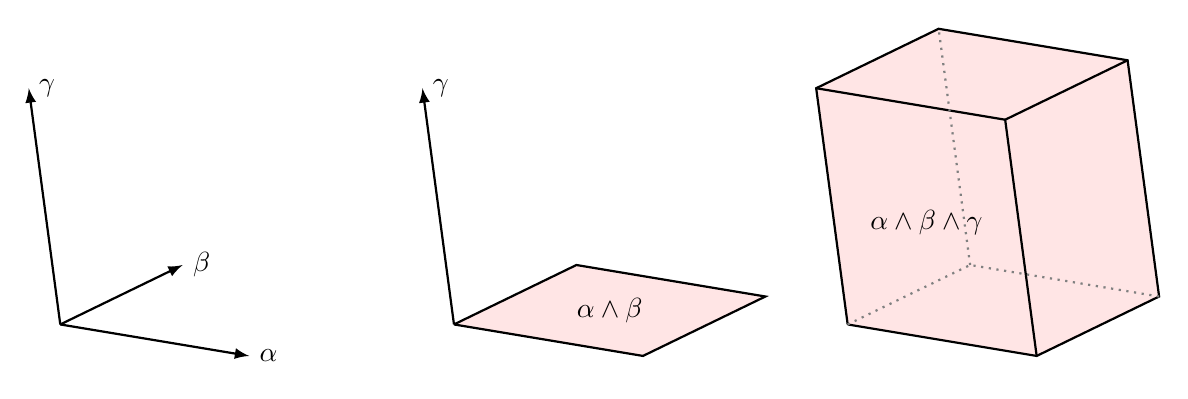
\begin{tikzpicture}[scale=2, thick]
    \coordinate (x) at (1.2, -0.2, 0);
    \coordinate (z) at (0.2, -0.2, -1.5);
    \coordinate (y) at (-0.2, 1.5, 0);
    \draw[->] (0,0,0) -- (x);
    \draw[->] (0,0,0) -- (z);
    \draw[->] (0,0,0) -- (y);
    \node[anchor=west] at (x) {$\alpha$};
    \node[anchor=west] at (z) {$\beta$};
    \node[anchor=west] at (y) {$\gamma$};

    \begin{scope}[xshift=2.5cm]
      \coordinate (x) at (1.2, -0.2, 0);
      \coordinate (z) at (0.2, -0.2, -1.5);
      \coordinate (y) at (-0.2, 1.5, 0);
      \draw[fill=red!10] (0,0,0) -- (x) -- ($(x) + (z)$) -- (z) -- (0,0,0);
      \draw[->] (0,0,0) -- (y);
      \node at ($0.5*(x) + 0.5*(z)$) {$\alpha \wedge \beta$};
      \node[anchor=west] at (y) {$\gamma$};
    \end{scope}

    \begin{scope}[xshift=5cm]
      \coordinate (x) at (1.2, -0.2, 0);
      \coordinate (z) at (0.2, -0.2, -1.5);
      \coordinate (y) at (-0.2, 1.5, 0);
      \fill[fill=red!10] (0,0,0) -- (x) -- ($(x) + (z)$) -- ($(x) + (y) + (z)$) -- ($(y) + (z)$) -- (y) -- (0,0,0);
      \draw (0,0,0) -- (x) -- ($(x) + (z)$) -- ($(x) + (y) + (z)$) -- ($(y) + (z)$) -- (y) -- (0,0,0);
      \draw (x) -- ($(x) + (y)$) -- ($(x) + (y) + (z)$);
      \draw (y) -- ($(x) + (y)$);
      \draw[gray,dotted] (0,0,0) -- (z) -- ($(x) + (z)$);
      \draw[gray,dotted] (z) -- ($(z) + (y)$);
      \node at ($0.5*(x) + 0.5*(y)$) {$\alpha \wedge \beta \wedge \gamma$};
    \end{scope}
  \end{tikzpicture}
  \caption{Exterior products of 1-forms visualized as volumes.}
  \label{fig:wedge}
\end{figure}

Thinking about an $n$-form as an oriented piece
of an $n$-dimensional subspace like this is an intuition
which will be useful in understanding the operations of exterior calculus.

Naturally, the dimension of a form cannot exceed that of the space it's embedded in.
Thus, the wedge product in $n$-dimensional space
is only defined for operands whose dimensions sum to $n$ or less.

A consequence of the wedge product being defined to measure volumes
(algebraically, a consequence of the antisymmetry equation \eqref{eq:wedge_antisymmetry})
is that the wedge product of a $k$-form with itself is zero when $k$ is odd;
\[
  \alpha \wedge \beta = -\beta \wedge \alpha
  \implies \alpha \wedge \alpha = 0.
\]
This is because, intuitively, two parallel vectors
form a parallelogram with zero area,
and in general a linearly dependent set of vectors
forms a degenerate volume.

On the other hand, when $k$ is even (including zero),
antisymmetry does not apply and $\alpha \wedge \alpha$ behaves like a dot product.
For 0-forms, whose wedge product is scalar multiplication,
this means $\alpha \wedge \alpha = \alpha^2$.
For higher-dimensional forms this only begins to apply in four dimensions,
where 2-forms can be multiplied.

Equipped with the exterior product,
we can define a basis for higher-dimensional forms.

\subsection{Higher-dimensional basis forms}\label{sec:basis_higher}

Basis forms of dimension 2 and above
are defined in terms of basis 1-forms and the exterior product.

In three dimensions, there are obviously three basis 1-forms.
The basis of 2-forms also has three elements,
or in other words, there are three linearly independent basis planes.
This number can be deduced algebraically
by taking the wedge product of all possible pairs of basis 1-forms
and eliminating ones that are either zero or a multiple of another.
A more intuitive geometric reasoning is that 
a plane in three dimensions is uniquely identified by its normal vector;
therefore the space of all planes has the same dimension as the space of all vectors.

There is only one three-dimensional subspace of three-dimensional space,
and thus only one basis 3-form.
This is true for any $n$:
there is only one basis $n$-form in $n$-dimensional space.
This form is called the \textit{volume form} of the space,
and it behaves like a scalar in computations.
Table \ref{tab:basis_3d} lists the basis forms in $\mathbb{R}^3$.

\begin{table}[h]
  \begin{tabular}{c | l}
    $n$ & basis $n$-forms \\
    \hline
    0 & 1 \\
    1 & $dx$,\, $dy$,\, $dz$ \\
    2 & $dx \wedge dy$,\, $dy \wedge dz$,\, $dz \wedge dx$ \\
    3 & $dx \wedge dy \wedge dz$ \\
  \end{tabular}
  \caption{Basis forms in $\mathbb{R}^3$.}
  \label{tab:basis_3d}
\end{table}

In two dimensions things are somewhat simpler,
as there is only one plane, and the 2-form is the volume form.
Table \ref{tab:basis_2d} lists the basis forms in $\mathbb{R}^2$.

\begin{table}[h]
  \begin{tabular}{c | l}
    $n$ & basis $n$-forms \\
    \hline
    0 & 1 \\
    1 & $dx$,\, $dy$ \\
    2 & $dx \wedge dy$ \\
  \end{tabular}
  \caption{Basis forms in $\mathbb{R}^2$.}
  \label{tab:basis_2d}
\end{table}

\subsection{Hodge star}\label{sec:hodge}

Consider the idea mentioned in section \ref{sec:basis_higher}
that a plane in three dimensions is uniquely identified by its normal vector.
This is one manifestation of the general fact that a linear subspace
is uniquely identified by its orthogonal complement.
In the context of differential forms,
an analogous statement is that there is an equal number
of basis $k$-forms and $(n-k)$-forms in $n$-dimensional space
and the map from a $k$-form to its orthogonal $(n-k)$-form
is an isomorphism.

The isomorphism taking a $k$-form to the orthogonal $(n-k)$-form
with the same magnitude is an important operator
called the \textit{Hodge star} $\star$.
It is a linear operator whose effect on the $\mathbb{R}^3$ basis forms
is as follows:

\begin{align*}
  \star 1 &= dx \wedge dy \wedge dz \\
  \star dx &= dy \wedge dz \\
  \star dy &= dz \wedge dx \\
  \star dz &= dx \wedge dy \\
  \star (dx \wedge dy) &= dz \\
  \star (dy \wedge dz) &= dx \\
  \star (dz \wedge dx) &= dy \\
  \star (dx \wedge dy \wedge dz) &= 1 \\
\end{align*}

Applying the star twice amounts to doing nothing at all,
$\star\star\alpha = \alpha$.

In $\mathbb{R}^2$ this is complicated slightly by the fact that
the orthogonal complement of a line is also a line,
and the Hodge star on 1-forms amounts to a 90 degree rotation.
Hence, for 1-forms in $\mathbb{R}^2$, a star twice is a 180 degree rotation,
$\star\star\alpha = -\alpha$.
In general, for $k$-forms in $n$-dimensional space,
\[
  \star\star\alpha = (-1)^{k(n-k)}\alpha.
\]

The effect of the Hodge star on the $\mathbb{R}^2$ basis forms is
\begin{align*}
  \star 1 &= dx \wedge dy \\
  \star dx &= dy \\
  \star dy &= -dx \\
  \star (dx \wedge dy) &= 1 \\
\end{align*}

TODO: Something about how
the Hodge star depends on the metric?
Something about the inner product?
These things aren't really relevant to the current use case,
but might be interesting

\subsection{Exterior derivative}\label{sec:ext_der}

The final operations we need to define the \textit{calculus} part of exterior calculus
are differentiation and integration.
Integration is exactly the procedure familiar from multivariate calculus
(differential forms are integrands, after all).
1-forms can be integrated over curves, 2-forms over surfaces,
3-forms over volumes, and so on.
Differentiation is performed by the \textit{exterior derivative} $\mathbf{d}$,
which, like the exterior product,
is equivalent to several different vector operators
depending on the dimension of its operand.

A common property of the exterior derivative regardless of dimension
is that it increases the dimension of its operand by one.
In other words, the exterior derivative of a $k$-form is a $(k+1)-form$.
This, along with the \textit{product rule}
\[
  \mathbf{d}(\alpha \wedge \beta)
  = \mathbf{d}\alpha \wedge \beta + (-1)^k \beta \wedge \mathbf{d}\alpha,
\]
the property $\mathbf{d} \circ \mathbf{d} = 0$,
and the definition of $\mathbf{d}$ for 0-forms,
can be used to recursively define the exterior derivative for all dimensions,
but as with the wedge product, the formal definition is very abstract.
An intuitive explanation of why $\mathbf{d}$ is defined this way
is outside the scope of this thesis,
but a reasoning based on the \textit{differential of a manifold}
is given in \cite{crane_digital_2013}.
For our purposes it will suffice to cover the equivalent vector proxy operations
for each dimension of $\mathbf{d}$.

A 0-form $f$ is a scalar function.
Its exterior derivative is the gradient, also known as the differential,
\[
  \mathbf{d}f = \nabla f = df.
\]
Omitting conversions with $\sharp$, $\flat$ and $\star$ for clarity,
the exterior derivative of a 1-form $\alpha$ corresponds to the
\textit{curl} of the vector proxy,
\[
  \mathbf{d}\alpha \eqsim \nabla \times \alpha.
\]
The exterior derivative of the volume form is not defined
(as it would produce a form of higher dimension than the space),
so in two dimensions this is the final $\mathbf{d}$.
In three dimensions, the exterior derivative of a 2-form $\beta$
is the \textit{divergence} of the (perpendicular) vector proxy,
\[
  \mathbf{d}\beta \eqsim \nabla \cdot \beta.
\]

These relationships give rise to \textit{Stokes' theorem},
which states that for a $k$-dimensional domain $\Omega$
with boundary $\partial \Omega$ and a $(k-1)$-form $\alpha$,

\begin{equation}\label{eq:stokes_theorem}
  \int_{\Omega} \mathbf{d}\alpha = \int_{\partial\Omega} \alpha.
\end{equation}

This theorem encapsulates several vector calculus identities
such as Green's theorem and the divergence theorem.
It is crucial in defining the discrete exterior calculus
and will be covered in more detail in section \ref{sec:disc_ext_der}.

More possible differential forms TODOs:
\begin{itemize}
  \item why this is useful: coordinate-free formulas (simplicity/conciseness),
    curved space, higher dimensional space
  \item manifolds?
\end{itemize}


\section{Computation mesh}

The discrete spatial structure at the root of the DEC is the \textit{simplicial complex}:
essentially a mesh (in the computer graphics sense)
consisting of triangles in two dimensions,
tetrahedra in three dimensions, or \textit{$k$-simplices} in $k$ dimensions.
We will focus on the two-dimensional case here for illustration.
This section is based on \parencite{desbrun_discrete_2006}.


\subsection{Simplices}

A \textit{$k$-simplex} is the simplest type of $k$-dimensional element
in a polyhedral mesh, defined as
the convex hull of $k + 1$ geometrically distinct points.
In concrete terms, a 0-simplex is a single point,
a 1-simplex is a line segment, a 2-simplex is a triangle,
a 3-simplex is a tetrahedron, and so on.
In the context of a mesh, a 0-simplex is often called a \textit{vertex},
a 1-simplex an \textit{edge}, a 2-simplex a \textit{face},
and a $k$-simplex where $k > 2$ a \textit{volume} or \textit{$k$-volume}.

Every simplex with dimension $k > 0$
has a \textit{boundary} consisting of $(k-1)$-simplices.
For instance, every triangle (2-simplex) is bounded by three line segments (1-simplices),
and every line segment is bounded by two vertices.
Each $(k-1)$-simplex on the boundary of a $k$-simplex $\sigma_k$
is called a \textit{$(k-1)$-face} of $\sigma_k$.

We denote simplices by listing their vertices, e.g. a triangle
$\sigma_2 = \{v_0, v_1, v_2\}$.


\subsection{Simplicial complex}

A simplicial complex $\mathcal{K}$ is a set of simplices satisfying the rules

\begin{itemize}
  \item every face of every simplex in $\mathcal{K}$ is also in $\mathcal{K}$
  \item any two simplices in $\mathcal{K}$ either do not intersect at all
    or share an entire face.
\end{itemize}

In the case of a 2D triangle mesh, this means
that every edge and vertex of every triangle is also part of the complex,
and there are no overlapping triangles
or edges/vertices that aren't part of a triangle's boundary.

A similar complex could be defined without requiring
all its elements to be simplicial.
For instance, a rectilinear grid is a common such structure.
A complex like this is called a \textit{cell complex}
and its $k$-dimensional elements \textit{$k$-cells}.
A simplex is a special case of a cell,
and the concepts of boundary and face apply to all cells.
We will use a simplicial complex in this thesis,
however, non-simplicial cells become relevant in the \textit{dual mesh}
(section \ref{sec:dual_mesh}).


\subsection{Orientation of a simplex}

Much like how differential forms of dimension 2 and higher
have a notion of two distinct orientations,
which manifest themselves in the sign of measured volumes,
simplices with 2 or more vertices also have two possible orientations
depending on the order of the vertices.
For a line segment there are two possible ways to order its two vertices,
for a triangle there are three clockwise and three counterclockwise orderings,
and so on.

As part of the definition of our simplicial complex,
each simplex receives an orientation.
For reasons that will become clear when
we define the discrete exterior derivative in section \ref{sec:disc_ext_der},
every simplex also needs its boundary to match its orientation.
For a counterclockwise oriented triangle, for instance,
this means the boundary line segments must form
a counterclockwise circulation around the triangle.
Since a line segment is often part of two triangles with conflicting orientations,
the defined orientations cannot be consistent with every boundary.

To resolve inconsistent face orientations,
the \textit{boundary operator} $\partial$,
which takes a simplex and returns its faces,
must flip every face that doesn't match the desired orientation.
This is denoted as a multiplication by -1.
For example, the boundary of a counterclockwise oriented triangle $\{v_0, v_1, v_2\}$
with edges $\{v_0, v_1\}$, $\{v_1, v_2\}$, $\{v_0, v_2\}$ is
\[
  \partial \{v_0, v_1, v_2\} = \{v_0, v_1\} + \{v_1, v_2\} - \{v_0, v_2\}.
\]

\begin{figure}[h]
  \centering
  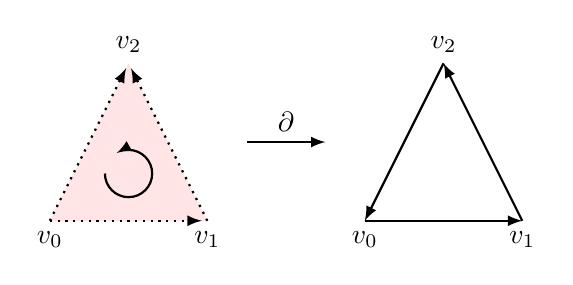
\begin{tikzpicture}
    \fill[fill=red!10] (-1,0) -- (1,0) -- (0,2);
    \draw[thick, dotted, -{>[sep=2pt]}] (-1,0) node[anchor=north]{$v_0$} -- (1,0);
    \draw[thick, dotted, -{>[sep=2pt]}] (1,0) node[anchor=north]{$v_1$} -- (0,2);
    \draw[thick, dotted, -{>[sep=2pt]}] (-1,0) -- (0,2) node[anchor=south]{$v_2$};
    \draw[thick, ->] (-0.3,0.6) arc (-180:120:0.3);

    \draw[thick, ->] (1.5, 1) -- node[anchor=south]{$\partial$} (2.5, 1);

    \draw[thick, ->] (3,0) node[anchor=north]{$v_0$} -- (5,0);
    \draw[thick, ->] (5,0) node[anchor=north]{$v_1$} -- (4,2);
    \draw[thick, ->] (4,2) node[anchor=south]{$v_2$} -- (3,0);
  \end{tikzpicture}
  \caption{
    \label{fig:triangle_boundary}
    Boundary of a triangle with inconsistently oriented faces.
  }
\end{figure}


\subsection{Chains and cochains}\label{sec:chains}

A \textit{$k$-chain} on a simplicial complex $\mathcal{K}$
is a set of real values associated with every $k$-simplex in $\mathcal{K}$.
Denoting the set of all $k$-simplices in $\mathcal{K}$ by $\mathcal{K}^k$
and its cardinality by $|\mathcal{K}^k|$,
a natural represenation for a chain is a $|\mathcal{K}^k|$-dimensional vector.
The space of all $k$-chains $\mathcal{C}_k$ is a vector space,
and the set of all $k$-simplices can be thought of as its basis.

Whereas a chain is analogous to a vector,
a \textit{cochain} is analogous to a differential form:
a linear function that takes a chain and ''measures'' it,
producing a real number.
A $k$-cochain $\omega^k$ has one linear operation for each $k$-simplex in $\mathcal{K}$,
matching the dimension of the corresponding $k$-chain $c_k$,
and the evaluation $\omega^k(c_k)$ behaves like an inner product between vectors.
Thus, a natural way to represent a cochain is a $|\mathcal{K}^k|$-dimensional \textit{row vector}.

This analogy with differential forms will be useful
when we define discrete forms in the next section.


\section{Discrete differential forms}

Equipped with an oriented simplicial complex,
we can begin to map differential forms and their operations onto it.
This section is based on \parencite{desbrun_discrete_2006},
\parencite{crane_digital_2013}, and \parencite{blair_perot_differential_2014}.


\subsection{Definition of discrete forms}\label{sec:discrete_forms}

Recalling that differential forms can be integrated
over manifolds of matching dimension,
a natural way to map a continuous form to a discrete value on a simplex
is to integrate the form over that simplex.
In other words, given a differential $k$-form $\omega^k$
and $k$-simplex $\sigma_k$, we can get a scalar value $\widehat{\omega}^k$
associated with $\sigma_k$ by computing the integral

\[
  \widehat{\omega}^k = \int_{\sigma_k} \omega^k.
\]

This is a line integral over a line segment for 1-forms,
surface integral over a triangle for 2-forms,
volume integral over a tetrahedron for 3-forms, and so on.
Additionally, a 0-form (i.e. a scalar field)
integrated over a 0-simplex (i.e. a single point)
is the value of the form at that point.

Computing this integral for every $k$-simplex in a simplicial complex $\mathcal{K}$
produces a set of values associated with the $k$-simplices,
which can be interpreted as a chain or cochain.
Due to the analogous nature of differential forms and cochains
covered in section \ref{sec:chains},
the most fitting choice of interpretation here is a cochain.
This leads us to the following definition:

A discrete differential $k$-form on an oriented simplicial complex $\mathcal{K}$
is a $k$-cochain obtained by integrating a continuous $k$-form
over every $k$-simplex in $\mathcal{K}$.

A consequence of defining discrete forms as a single real value per simplex
is that vector-valued forms (1-forms and 2-forms in 3D)
lose information about their direction.
A line integral only records the component of the form tangential to the line,
discarding the orthogonal component,
and a surface integral is only affected by flux across the surface.
However, directions are not actually needed in most DEC computations.
If one is desired (e.g. for visualization),
it can be reconstructed from multiple nearby simplices via \textit{interpolation},
which will be covered in section \ref{sec:interpolation}.

TODO: that last paragraph is maybe a bit confusing,
can I word it better or move it somewhere else?
Could be best to just say this in the interpolation section
without alluding to it beforehand

The discrete equivalent of a differential form being a cochain,
the discrete versions of the operations of exterior calculus
are operations on cochains.

\subsection{Discrete exterior derivative}\label{sec:disc_ext_der}

Section \ref{sec:ext_der} briefly introduced Stokes' theorem
(equation \ref{eq:stokes_theorem}).
In the domain of a $k$-simplex $\sigma$, it states that
\begin{equation}\label{eq:stokes_simplex}
  \int_{\sigma} \mathbf{d}\alpha = \int_{\partial\sigma} \alpha,
\end{equation}
where $\alpha$ is a $(k-1)$-form.

Writing this in terms of the exterior derivative's
vector analogues covered in section \ref{sec:ext_der}
($\nabla$, $\nabla \times$, and $\nabla \cdot$)
yields several well-known vector calculus identities.

When $k = 1$, equation \ref{eq:stokes_simplex}
is the fundamental theorem of calculus
\begin{equation}\label{eq:fund_theorem_calc}
  \int_{\sigma} \nabla \alpha = \alpha(v_2) - \alpha(v_1)
\end{equation}
where $v_1,v_2$ are the endpoints of the line segment $\sigma$.

When $k = 2$, we get the curl theorem
\begin{equation}\label{eq:curl_theorem}
  \iint_{\sigma} (\nabla \times \alpha) \cdot dA = \int_{\partial\sigma} \alpha \cdot dl,
\end{equation}
which is equivalent to Green's theorem in two-dimensional space.

Finally, when $k = 3$, we get the divergence theorem
\begin{equation}\label{eq:divergence_theorem}
  \iiint_{\sigma} (\nabla \cdot \alpha) \,dV = \iint_{\partial\sigma} \alpha \,dA.
\end{equation}

Stokes' theorem expresses and generalizes the common property between these identities,
that an integral over a $k$-dimensional volume
can be turned into an integral over the volume's boundary and vice versa.
It is a powerful theorem with many applications.
For the use case of discrete exterior calculus,
it can be used as the \textit{definition} of
the discrete exterior derivative.
More specifically, we can define the discrete exterior derivative
as the unique operator $\mathbf{d}$ satisfying equation \ref{eq:stokes_simplex}.

To make this concrete, first note that the integrals here
are exactly how cochain elements were defined in section \ref{sec:discrete_forms}.
$\int_{\sigma} \mathbf{d}\alpha$ is an element of a $k$-cochain,
and $\int_{\partial\sigma} \alpha$ is the sum of all $(k-1)$-cochain elements
constituting the boundary of $\sigma$.
In a sense, $\mathbf{d}$ does the opposite of the boundary operator $\partial$
defined in section \ref{sec:discrete_forms}:
whereas $\partial$ takes a simplex and produces the sum of its faces,
$\mathbf{d}$ takes the sum of a simplex's faces and produces the simplex itself.
In more precise terms, $\mathbf{d}$ is the \textit{adjoint} of $\partial$,
also known as the \textit{coboundary operator}.

Given a simplicial complex $\mathcal{K}$,
$\mathbf{d}$ is a linear map from $\mathcal{K}^{k-1}$ to $\mathcal{K}^k$.
Hence, it can be represented as a $|\mathcal{K}^k| \times |\mathcal{K}^{k-1}|$ matrix.
Each row of this matrix corresponds to one $k$-simplex
and represents a signed sum of its faces taking into account relative orientation.
Each column corresponding to a boundary simplex has a coefficient
of 1 or -1 depending on orientation,
and the rest of the coefficients are zeroes.
Graph theorists call this type of matrix an \textit{adjacency matrix}.

Figure \ref{fig:discrete_ext_derivative} illustrates
the discrete exterior derivative on a small simplicial complex.
The subscript on $\mathbf{d}$ denotes the dimension of the input cochain,
and the numbers in the diagrams represent the index of the mesh element in the cochain.
The triangle faces are all oriented counterclockwise.

\begin{figure}[h]
  \centering
  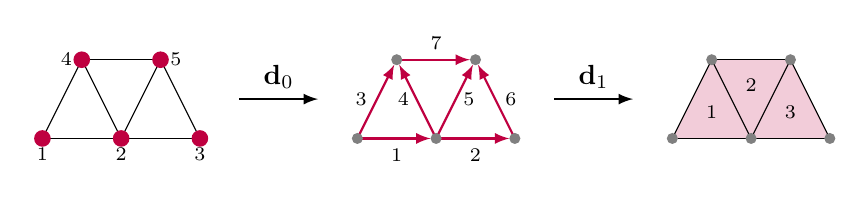
\begin{tikzpicture}
    \draw (0,0) -- (1,0);
    \draw (1,0) -- (2,0);
    \draw (0,0) -- (0.5,1);
    \draw (1,0) -- (0.5,1);
    \draw (1,0) -- (1.5,1);
    \draw (2,0) -- (1.5,1);
    \draw (0.5,1) -- (1.5,1);
    \begin{scope}[font=\scriptsize, fill=purple]
      \fill (0,0) circle (3pt) node[anchor=north]{1};
      \fill (1,0) circle (3pt) node[anchor=north]{2};
      \fill (2,0) circle (3pt) node[anchor=north]{3};
      \fill (0.5,1) circle (3pt) node[anchor=east]{4};
      \fill (1.5,1) circle (3pt) node[anchor=west]{5};
    \end{scope}
    
    \draw[thick, ->] (2.5, 0.5) -- node[anchor=south]{$\mathbf{d}_0$} (3.5,0.5);

    \begin{scope}[xshift=4cm]
      \begin{scope}[thick, font=\scriptsize, draw=purple, -{>[sep=2pt]}]
        \draw (0,0) -- node[below]{1} (1,0);
        \draw (1,0) -- node[below]{2} (2,0);
        \draw (0,0) -- node[left]{3} (0.5,1);
        \draw (1,0) -- node[left=-1pt]{4} (0.5,1);
        \draw (1,0) -- node[right=-1pt]{5} (1.5,1);
        \draw (2,0) -- node[right]{6} (1.5,1);
        \draw (0.5,1) -- node[above]{7} (1.5,1);
      \end{scope}
      \begin{scope}[gray]
        \fill (0,0) circle (2pt);
        \fill (1,0) circle (2pt);
        \fill (2,0) circle (2pt);
        \fill (0.5,1) circle (2pt);
        \fill (1.5,1) circle (2pt);
      \end{scope}
      
      \draw[thick, ->] (2.5, 0.5) -- node[anchor=south]{$\mathbf{d}_1$} (3.5,0.5);
    \end{scope}

    \begin{scope}[xshift=8cm]
      \fill[fill=purple!20] (0,0) -- (2,0) -- (1.5,1) -- (0.5,1);
      \draw (0,0) -- (1,0);
      \draw (1,0) -- (2,0);
      \draw (0,0) -- (0.5,1);
      \draw (1,0) -- (0.5,1);
      \draw (1,0) -- (1.5,1);
      \draw (2,0) -- (1.5,1);
      \draw (0.5,1) -- (1.5,1);
      \begin{scope}[gray]
        \fill (0,0) circle (2pt);
        \fill (1,0) circle (2pt);
        \fill (2,0) circle (2pt);
        \fill (0.5,1) circle (2pt);
        \fill (1.5,1) circle (2pt);
      \end{scope}
      \begin{scope}[font=\scriptsize]
        \node at (0.5,0.33) {1};
        \node at (1,0.67) {2};
        \node at (1.5,0.33) {3};
      \end{scope}
    \end{scope}
  \end{tikzpicture}
  \caption{Discrete exterior derivative visualized on an oriented simplicial complex.}
  \label{fig:discrete_ext_derivative}
\end{figure}

TODO: is this still too many edges to keep the matrices readable?
Should I remove one more vertex?

The matrix representations of $\mathbf{d}_0$ and $\mathbf{d}_1$
in figure \ref{fig:discrete_ext_derivative} are

\[
  \mathbf{d}_0 = \begin{bmatrix}[0.8]
    -1 & 1 \\
       & -1 & 1 \\
    -1 & & & 1 \\
       & -1 & & 1 \\
       & -1 & & & 1 \\
       & & -1 & & 1 \\
       & & & -1 & 1 \\
  \end{bmatrix},
  \qquad
  \mathbf{d}_1 = \begin{bmatrix}[0.8]
    1 & & -1 & 1 \\
      & & & -1 & 1 & & -1 \\
      & 1 & & & -1 & 1 \\
  \end{bmatrix}.
\]

A remarkable property of a discrete exterior derivative
defined this way is that it is \textit{exact}.
The value obtained by integrating a form over boundary simplices
and taking the discrete exterior derivative
is exactly the value one would obtain
by first taking the continuous exterior derivative of the same form
and integrating it over the bounded volume.
As a result, use of the discrete exterior derivative in a numerical method
introduces no additional error.
This simplifies the analysis of a method's accuracy
by eliminating one source of error.

TODO: unify notation: pick either $\alpha$ or $\omega$
and use it for all forms and cochains,
and either use or don't use dimension indices.
Also consider removing the hat notation for cochains,
since the hat notation is also used for complex values
in the harmonic timestepping section

\subsection{Dual mesh}\label{sec:dual_mesh}

The continuous Hodge star is an isomorphism
that maps a $k$-form to an orthogonal $(n-k)$-form.
To capture these notions of isomorphism and orthogonality
in the discrete setting, a simplicial complex alone is insufficient.
Some additional geometric structure is needed.

Given a simplicial complex $\mathcal{K}$,
a secondary complex constructed for the purpose of the discrete Hodge star
is called a \textit{dual mesh}, denoted $\mathcal{K}^*$.
When the dual relationship is relevant,
$\mathcal{K}$ is in turn called the \textit{primal mesh}.

The most important property of the dual mesh
is that every $k$-simplex in $\mathcal{K}$
has a corresponding $(n-k)$-cell in $\mathcal{K}^*$.
In two dimensions this means every primal vertex maps to a dual face,
every primal edge maps to a dual edge, and every primal face maps to a dual vertex.
This is illustrated in figure \ref{fig:dual_mesh},
with the purple dotted lines representing the dual mesh.

\begin{figure}[h]
  \centering
  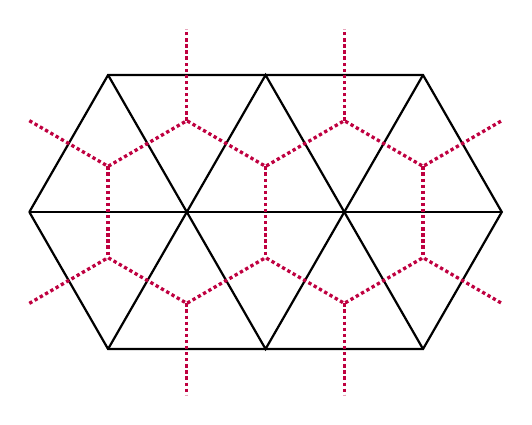
\begin{tikzpicture}[scale=2, thick]
    \draw (0,0) -- (3,0);
    \draw (0,0) -- (0.5,-0.87) -- (2.5,-0.87) -- (3,0) -- (2.5,0.87) -- (0.5,0.87) -- (0,0);
    \draw (0.5,-0.87) -- (1.5,0.87) -- (2.5,-0.87);
    \draw (0.5,0.87) -- (1.5,-0.87) -- (2.5,0.87);

    \begin{scope}[purple, densely dotted, very thick]
      \draw (0,0.58) -- (0.5,0.29) -- (1,0.58) -- (1.5,0.29) -- (2,0.58) -- (2.5,0.29) -- (3,0.58);
      \draw (0,-0.58) -- (0.5,-0.29) -- (1,-0.58) -- (1.5,-0.29) -- (2,-0.58) -- (2.5,-0.29) -- (3,-0.58);
      \draw (0.5,0.29) -- (0.5,-0.29);
      \draw (1.5,0.29) -- (1.5,-0.29);
      \draw (2.5,0.29) -- (2.5,-0.29);
      \draw (1,0.58) -- (1,1.16);
      \draw (2,0.58) -- (2,1.16);
      \draw (1,-0.58) -- (1,-1.16);
      \draw (2,-0.58) -- (2,-1.16);
    \end{scope}
  \end{tikzpicture}
  \caption{A mesh and its dual.}
  \label{fig:dual_mesh}
\end{figure}

Notably, a dual mesh is generally not a simplicial one.
For instance, a regular triangular grid in 2D,
such as the one in figure \ref{fig:dual_mesh}, will have hexagonal dual faces.
However, the boundary operator and discrete exterior derivative
are defined in a way that can handle arbitrary polytopes.
The number of faces on a cell merely affects the sparsity pattern
of the matrix $\mathbf{d}$.

A somewhat more challenging property of the dual mesh
are its incomplete faces on the boundary.
For instance, the dual mesh of figure \ref{fig:dual_mesh} has two hexagonal faces
and eight edges pointing outside the primal mesh, connected to nothing at the outer end.
Care must be taken to account for this when defining boundary conditions.
An example of appropriately defined boundary conditions
will be given in section \ref{sec:boundary_conditions}.

There are many possible ways to place the dual elements relative to the primal ones.
In this thesis, \textit{circumcentric} dual cells 
as implemented by the PyDEC software library \parencite{bell_pydec_2012} are used,
meaning the dual vertex of a primal $n$-simplex
is placed at the center of the smallest $n$-ball containing the simplex,
or in other words, at the point that is equidistant from
all vertices of the simplex.
An important property of a dual mesh defined this way is
that primal and dual elements are orthogonal to one another.

\subsection{Discrete Hodge star}

The discrete Hodge star is a mapping between $k$-cochains on the primal mesh
and $(n-k)$-cochains on the dual mesh.
By construction of the dual mesh,
this mapping in matrix form is a square $(|\mathcal{K}^k| \times |\mathcal{K}^k|)$-matrix.
For efficient computation, it is desirable for this matrix to be diagonal,
as diagonal matrices are fast to multiply and trivial to invert.

The Hodge star is diagonal when each element of the resulting dual cochain
only depends on its corresponding primal element.
The value of the diagonal elements is based on the idea
that the Hodge star produces a form of equal magnitude.
As we don't generally know the exact form the star will be applied to,
this necessarily involves approximation.

Given a continuous $k$-form $\alpha$, primal $k$-simplex $\sigma$,
and its dual $(n-k)$-cell $\sigma^*$,
a simple approximation for the discrete Hodge star
is obtained by assuming $\alpha$ is constant over $\sigma$ and $\sigma^*$.
Combined with the fact that $\alpha$ and $\star\alpha$ have equal magnitude,
this approximation leads to the idea that the cochains
$\hat{\alpha} = \int_{\sigma} \alpha$ and $\star\hat{\alpha} = \int_{\sigma^*} \star\alpha$
should have equal magnitude \textit{per unit of volume},
\[
  \frac{1}{|\sigma|} \hat{\alpha} = \frac{1}{|\sigma^*|} \star\hat{\alpha}
  \iff \star\hat{\alpha} = \frac{|\sigma^*|}{|\sigma|} \hat{\alpha}.
\]

A discrete Hodge star defined using this approximation
is a square diagonal matrix whose elements are
\begin{equation}
  \star_{ii} = \frac{|\sigma_i^*|}{|\sigma_i|}, \quad i = 1, \dots, |\mathcal{K}^k|.
\end{equation}

This approximation, which we call \textit{Yee's Hodge star}
due to its early appearance in \textcite{yee_numerical_1966},
is one of two Hodge star operators used in this thesis.
A different approximation is obtained by assuming spatially harmonic forms
instead of locally constant ones.
The details of this will be covered in section \ref{sec:harmonic_timestep}.

Because the discrete exterior derivative is exact,
the Hodge star is the only source of approximation error
in methods based on these two operators.
As such, variants of the discrete Hodge star directly lead to
DEC variants with different accuracy and efficiency characteristics.
Examples of this are the harmonic Hodge star used in this thesis
and the higher order approximations studied by \textcite{lohi_higher_2023}.

\subsection{Interpolating discrete forms}\label{sec:interpolation}

All values in DEC computations are cochains
and thus exist only on elements of a mesh.
However, it is sometimes useful to get the value of a form at a single point.
In this thesis, for instance, we would like to visualize
the 1-form velocity as arrows pointing in the direction of velocity,
but a 1-cochain has no notion of direction.
It only has magnitudes over entire mesh edges.
Thus, direction must be reconstructed by interpolating between multiple nearby edges.
This is accomplished using \textit{Whitney forms},
first introduced by \textcite{whitney_geometric_1957}.
This section gives a short summary of their definition;
see e.g. \textcite{lohi_whitney_2021} for a thorough treatment of the topic.

Whitney forms are defined individually for every simplex
in terms of \textit{barycentric coordinates}:
for a $k$-simplex with vertices $v_0, \dots, v_k$,
any point within the simplex can be expressed as
\[
  \sum_{i=0}^k \lambda_i v_i
\]
where the coefficients $\lambda_i$ are called barycentric coordinates.
If $\sum_{i=0}^k \lambda_i = 1$, these coordinates are called \textit{normalized}.
Equivalently to normalized barycentric coordinates,
the \textit{barycentric function} $\lambda_i$ for a vertex $v_i$
is a piecewise linear function whose value is 1 on $v_i$
and zero on all other vertices.

The Whitney form $\mathcal{W}$ associated with a 0-simplex $v_i$
is its barycentric function,
\[
  \mathcal{W}(v_i) = \lambda_i.
\]
For a 1-simplex $\sigma = [v_0,v_1]$, it is
\[
  \mathcal{W}(\sigma) = \lambda_0 d\lambda_1 - \lambda_1 d\lambda_0
\]
or equivalently in vector calculus notation,
\[
  \mathcal{W}(\sigma) = \lambda_0 \nabla\lambda_1 - \lambda_1 \nabla\lambda_0,
\]
and generally for a $k$-simplex $\sigma = [v_0,\dots,v_k]$,
\begin{equation}
  \mathcal{W}(\sigma) = k! \sum_{i=0}^{k} (-1)^i
    \lambda_i d\lambda_1 \wedge \dots \wedge \widehat{d\lambda_i}
    \wedge \dots d\lambda_k
\end{equation}
where $\widehat{\quad}$ denotes that the term is omitted.

Summing these forms across an entire simplicial complex $\mathcal{K}$
produces a piecewise smooth interpolating function called the \textit{Whitney map},
also (somewhat confusingly) denoted $\mathcal{W}$.
Given a $k$-cochain $\hat{\alpha}$ on $\mathcal{K}$ whose element $a_i$
is associated with the $k$-simplex $\sigma_i$,
the $k$-form Whitney map for $\mathcal{K}$ is
\begin{equation}
  \mathcal{W}(\hat{\alpha})
  = \mathcal{W}(\sum_{\sigma_i \in \mathcal{K}^k} a_i\sigma_i)
  = \sum_{\sigma_i \in \mathcal{K}^k} a_i \mathcal{W}(\sigma_i)
\end{equation}

Concretely, to evaluate the $k$-form Whitney map for a point $x$,
one would first find the $n$-simplex $x$ lies in
(since all the barycentric functions and hence the Whitney forms
for all simplices outside of it are zero),
where $n$ is the dimension of the working space,
find all the $k$-simplices that are faces of this $n$-simplex,
and sum their respective Whitney forms at $x$.
The use case in this thesis is interpolation of 1-forms in $\mathbb{R}^2$,
in which case one would find the triangle $x$ lies in
with sides $\sigma_0,\sigma_1,\sigma_2$
and associated cochain elements $a_0,a_1,a_2$,
and take the sum
\[
  a_0 (\mathcal{W}(\sigma_0))(x)
  + a_1 (\mathcal{W}(\sigma_1))(x)
  + a_2 (\mathcal{W}(\sigma_2))(x).
\]


\chapter{Model}\label{cha:model}

The physical phenomenon we apply the DEC to
is the propagation and scattering of acoustic waves
in a two-dimensional domain.
This chapter will cover the mathematical models used;
the details of numerical experiments performed and their results
are described in chapter \ref{cha:experiments}.

\section{Vector equations}

We consider waves described by the differential equation

\begin{equation}
  \frac{\partial^2 \phi}{\partial t^2} - c^2 \nabla^2\phi = 0
\end{equation}

where $\phi$ is a velocity potential, $t$ is time
and $c$ is the speed of wave propagation.
This equation is equivalent to the first-order system

\begin{equation}\label{eq:wave1stOrd}
  \begin{cases}
    \frac{\partial p}{\partial t} - c^2\nabla \cdot \mathbf{v} = 0 \\
    \frac{\partial \mathbf{v}}{\partial t} - \nabla p = 0 \\
  \end{cases}
\end{equation}

where $p = \frac{\partial \phi}{\partial t}$ is the scalar-valued acoustic pressure
and $\mathbf{v} = \nabla \phi$ is the vector-valued velocity
of particles perturbed by the wave.

The system \eqref{eq:wave1stOrd} applies within the spatial domain $\Omega$
and the time domain $[0, T]$.

\section{Exterior calculus equations}

The first step to translating the vector system \eqref{eq:wave1stOrd}
to exterior calculus notation is the selection of appropriate differential forms
to represent the variables $p$ and $\mathbf{v}$.
Because a scalar can be represented either by a 0-form or a volume form,
and a vector by a 1-form or $(n-1)$-form,
there are two possible choices for each variable,
both of which can be made equivalent to the vector equations
by the application of Hodge stars when necessary.
The physical properties of a variable can hint at the most appropriate choice,
but one can also begin with 0- and 1-forms
and pick the most convenient representation for the end result.

We begin by representing pressure with the 0-form $p$
and velocity with the 1-form $v = \mathbf{v}^{\flat}$.
The exterior derivative of a 1-form corresponds to the curl $\nabla \times$,
but we need the divergence of $v$ in the first equation of \eqref{eq:wave1stOrd}.
In three dimensions, divergence is the exterior derivative of a 2-form,
meaning computing the divergence of a 1-form involves first converting
it to a 2-form with a Hodge star, $\nabla \cdot \mathbf{v} \eqsim \mathbf{d}\star v$.
The equivalent turns out to be true in 2D as well.

To illustrate why, figure \ref{fig:2d_divergence} invokes Stokes' theorem.
Divergence integrated over an area is equal to the boundary curve integral
in the outward-pointing normal direction.
Curl, on the other hand, is the boundary curve integral in the tangent direction.
Thus, we can compute divergence by first rotating such that the boundary normal
points in the tangent direction, which is exactly the effect of the 1-form Hodge star,
and then taking the curl, i.e. the exterior derivative.

\begin{figure}[h]
  \centering
  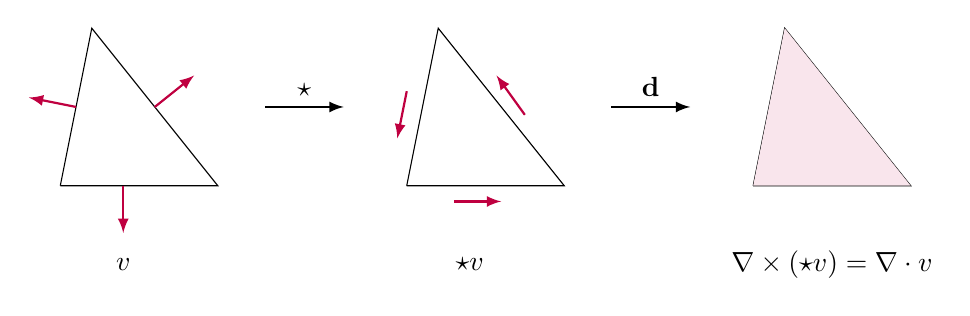
\begin{tikzpicture}[scale=2]
    \draw (0,0) -- (1,0) -- (0.2, 1) -- (0,0);
    \begin{scope}[thick,purple,->]
      \draw (0.4,-0.0) -- (0.4,-0.3);
      \draw (0.6,0.5) -- (0.85,0.7);
      \draw (0.1,0.5) -- (-0.2,0.56);
    \end{scope}
    \node at (0.4, -0.5) {$v$};
    \draw[thick,->] (1.3,0.5) -- node[above]{$\star$} (1.8,0.5);
    \begin{scope}[xshift=2.2cm]
      \draw (0,0) -- (1,0) -- (0.2, 1) -- (0,0);
      \begin{scope}[thick,purple,->]
        \draw (0.3,-0.1) -- (0.6,-0.1);
        \draw (0.75,0.45) -- (0.57,0.7);
        \draw (0.0,0.6) -- (-0.06,0.3);
      \end{scope}
      \node at (0.4,-0.5) {$\star v$};
      \draw[thick,->] (1.3,0.5) -- node[above]{$\mathbf{d}$} (1.8,0.5);
    \end{scope}
    \begin{scope}[xshift=4.4cm]
      \draw (0,0) -- (1,0) -- (0.2, 1) -- (0,0);
      \fill[purple!10] (0,0) -- (1,0) -- (0.2, 1) -- (0,0);
      \node at (0.5,-0.5) {$\nabla \times (\star v) = \nabla \cdot v$};
    \end{scope}
  \end{tikzpicture}
  \caption{2D divergence as the exterior derivative of a rotated form.}
  \label{fig:2d_divergence}
\end{figure}

Note that divergence expressed this way is a 2-form,
and we've chosen to represent $p$ as a 0-form.
To match the dimension of $p$, an additional Hodge star
needs to be applied to the divergence.
The first equation in \ref{eq:wave1stOrd} thus becomes
\begin{equation}\label{eq:intermediate_eq_1}
  \frac{\partial p}{\partial t} - c^2 \star \mathbf{d} \star v = 0.
\end{equation}

The second equation is more straightforward,
as the exterior derivative of a 0-form directly corresponds to the gradient.
In exterior calculs notation, it becomes
\begin{equation}\label{eq:intermediate_eq_2}
  \frac{\partial v}{\partial t} - \mathbf{d} p = 0.
\end{equation}

These equations are a good starting point, but we're not quite finished yet.
The problem arises from the absorbing boundary condition,
which will be covered in more detail in section \ref{sec:boundary_conditions}.
The boundary condition involves the \textit{flux} of velocity across the boundary,
meaning its component normal to the boundary, $\mathbf{v} \cdot \mathbf{n}$.
If we represent $v$ as a 1-cochain, integrating $v$ over boundary edges
in the tangent direction, information about the normal direction is lost.
Thus, to express this boundary condition,
we need to represent our equations in terms of flux instead of velocity.

In exterior calculus notation the flux is $\star v$.
The reason for this is the same as the reason
why divergence can be computed as the curl of $\star v$.
In a sense, the star turns a line integrated in the tangent direction
into a line integrated in the normal direction,
analogously to the 3D case where a 1-form (line)
turns into a 2-form (surface) integrated in the normal direction.

The final choices for the unknowns in our equations
are the 0-form pressure $p$
and the 1-form velocity flux $q = \star v$.
Substituting these variables into equations \eqref{eq:intermediate_eq_1}
and \eqref{eq:intermediate_eq_2} and applying one more Hodge star 
to \eqref{eq:intermediate_eq_2} yields the system
\begin{equation}
  \begin{cases}
    \frac{\partial p}{\partial t} - c^2 \star \mathbf{d} q = 0 \\
    \frac{\partial q}{\partial t} - \star \mathbf{d} p = 0 \\
  \end{cases}
\end{equation}

\section{Discretization}

Discretization of the model into a computer-solvable form
is performed separately for space and time.
The procedures defined by DEC are used for the spatial part,
and time discretization is performed using a staggered
finite difference scheme known as the leapfrog method.

\subsection{Space}

Spatial discretization in DEC is straightforward:
given a continuous model in exterior calculus notation,
a simplicial complex $\mathcal{K}$ approximating the domain $\Omega$ and its dual,
replace $k$-forms in the model with $k$-cochains,
$\mathbf{d}$ with the coboundary operator,
and $\star$ with the discrete Hodge star,
and you're most of the way done.
Denoting the 0-cochain equivalent of $p$ by $P$
and the 1-cochain equivalent of $q$ by $Q$,
this yields the semi-discrete equations
\begin{equation}\label{eq:semi_discrete_model}
  \begin{cases}
    \frac{\partial P}{\partial t} - c^2 \star \mathbf{d} Q = 0 \\
    \frac{\partial Q}{\partial t} - \star \mathbf{d} P = 0 \\
  \end{cases}
\end{equation}
(only \textit{semi}-discrete at this point
because they are still continuous in time).

The only remaining question is whether the cochains should be placed
on the primal mesh or the dual.
In our case, the implementation of boundary conditions demands $Q$
be available on the boundary edges, which means $Q$ must be on primal edges
(as dual edges are orthogonal to the boundary instead).
From there, $P$ should be placed such that the terms in equations \eqref{eq:semi_discrete_model}
are in the same cochain space.
In the first equation, $\star\mathbf{d}Q$
takes $Q$ from primal edges to primal faces and from there to dual vertices,
suggesting that $P$ should be a \textbf{dual} 0-cochain.
Checking that $\star \mathbf{d} P$ in the second equation
is a primal 1-cochain confirms this as the correct choice.

To produce the cochain elements $P_i$ and $Q_i$
on the dual vertices $v_i^*$ and primal edges $\mathcal{E}_i$
from the continuous variables $p$ and $\mathbf{v}$,
we get the formulas
\begin{align}
  \label{eq:cochain_p}
  P_i &= p(v_i^*) \\
  \label{eq:cochain_q}
  Q_i &= \int_{\mathcal{E}_i} (\mathbf{v} \cdot \mathbf{n}) \,dl.
\end{align}
Note the term $\mathbf{v} \cdot \mathbf{n}$ turning velocity into flux in \eqref{eq:cochain_q}.

TODO: should I mention the matrix form of eq. \eqref{eq:semi_discrete_model}?
Or just leave $\Lambda$ out of the exact controllability section
since it's the identity matrix?

\subsection{Time}

TODO: mention some sources of leapfrog scheme here? Räbinä's thesis lists a bunch

The leapfrog method for time discretization is a first-order finite difference scheme.
Time advances in steps of $\Delta t$ seconds,
and values of $P$ and $Q$ are computed at separate time instances
offset from each other by $\frac{\Delta t}{2}$.
Let $t^k = k\Delta t$ denote the value of time after $k$ timesteps
and $P^k$ the value of $P$ at this time.
The next value of $Q$ is computed at the time $t^k + \frac{\Delta t}{2}$,
which we denote $Q^{k+\frac{1}{2}}$.
The time derivatives of $P$ and $Q$ are then approximated with
\begin{eqnarray}
  \label{eq:time_derivative_p}
  \frac{\partial P}{\partial t}(t^{k+\frac{1}{2}}) = \frac{P^{k+1} - P^k}{\Delta t} \\
  \label{eq:time_derivative_q}
  \frac{\partial Q}{\partial t}(t^k) = \frac{Q^{k+\frac{1}{2}} - Q^{k-\frac{1}{2}}}{\Delta t}
\end{eqnarray}

Substituting \eqref{eq:time_derivative_p} and \eqref{eq:time_derivative_q}
into \eqref{eq:semi_discrete_model} yields
\begin{align*}
\frac{P^{n+1} - P^n}{\Delta t} - c^2 \star \mathbf{d} Q^{n+\frac{1}{2}} &= 0 \\
\frac{Q^{n+\frac{3}{2}} - Q^{n+\frac{1}{2}}}{\Delta t}
- \star \mathbf{d} P^{n+1} &= 0 \\
\end{align*}

TODO: I should probably write down the dimension subscripts,
inverse of Hodge star, and transpose of $\mathbf{d}$ like I did in my notes.
Here's how this looked there:
\begin{align*}
  \frac{P^{n+1} - P^n}{\Delta t} - c^2 \star_2 d_1 Q^{n+\frac{1}{2}} &= F \\
  \frac{Q^{n+\frac{3}{2}} - Q^{n+\frac{1}{2}}}{\Delta t}
  - \star_1^{-1} d_1^T P^{n+1} &= 0
\end{align*}
(first explain this notation in the theory section
and add it to the model section)

Multiplying by $\Delta t$ and moving terms to the right-hand side
produces the timestep formulas
\begin{align}
  P^{n+1} &= P^n + \Delta t c^2 \star \mathbf{d} Q^{n+\frac{1}{2}} \\
  Q^{n+\frac{3}{2}} &= Q^{n+\frac{1}{2}} + \Delta t \star \mathbf{d} P^{n+1}
\end{align}

This is an \textit{explicit} method:
the timestep formulas can be applied as matrix multiplications
to the values of $P$ and $Q$ at the beginning of a timestep,
without being required to solve any linear systems.

TODO: something about stability here?

\section{Boundary conditions}\label{sec:boundary_conditions}

Our main test case models the scattering of acoustic waves
on impact with a sound-soft obstacle.
(TODO: what does sound-soft mean. Hard to find a source actually defining this,
best I can find is "zero impedance" which doesn't really help intuition.
Does this mean waves travel through the boundary without changing in any way?)
For this purpose we define two boundaries,
$\Gamma_{sca}$ for the scattering obstacle
and $\Gamma_{ext}$ for the outer boundary of the computational domain,
illustrated in figure \ref{fig:scatterer_domain}.

\begin{figure}[h]
  \centering
  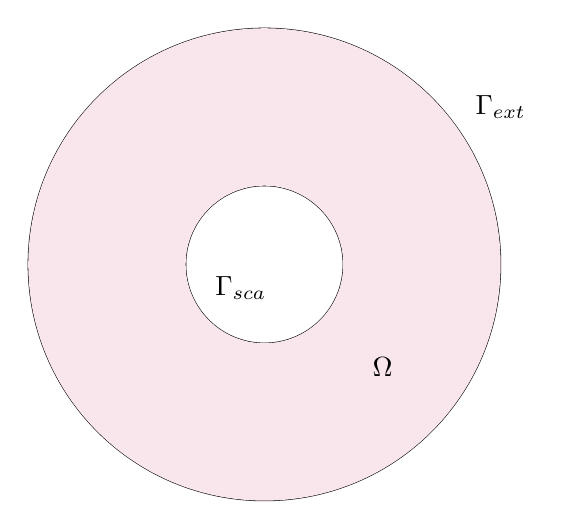
\begin{tikzpicture}
    \draw circle [radius=3];
    \draw circle [radius=1];
    \fill[fill=purple!10, even odd rule] circle [radius=3] circle [radius=1];
    \node at (3,2) {$\Gamma_{ext}$};
    \node at (-0.3,-0.3) {$\Gamma_{sca}$};
    \node at (1.5,-1.3) {$\Omega$};
  \end{tikzpicture}
  \caption{The domain $\Omega$ and boundaries $\Gamma_{ext}$ and $\Gamma_{sca}$
    of a scattering model.}
  \label{fig:scatterer_domain}
\end{figure}

Given an incoming wave with velocity potential $\phi_{inc}$,
the scattering obstacle is modelled by setting $\phi_{inc}$ on $\Gamma_{sca}$
as a Dirichlet boundary condition
\begin{equation}
  \mathbf{v} = \nabla \phi_{inc}
  \quad \text{in } \Gamma_{sca} \times [0, T].
\end{equation}
where $[0,T]$ is the simulated time period.
The boundary condition is only applied to $\mathbf{v}$
and not $p$ because $p$ is placed on the dual mesh,
which does not have elements at the boundary.

On the outer boundary of the domain $\Gamma_{ext}$
we want the waves to travel out of the domain uninterrupted
in order to model the domain sitting inside a larger empty space.
This is accomplished using a first-order absorbing Engqvist-Majda boundary condition
\parencite{engquist_absorbing_1977}
\[
  \frac{1}{c}\frac{\partial\phi}{\partial t} + \mathbf{n} \cdot \nabla\phi = 0
  \quad \text{in } \Gamma_{ext} \times [0, T].
\]

Substituting the variables $p = \frac{\partial \phi}{\partial t}$
and $\mathbf{v} = \nabla \phi$ yields
\[
  \frac{1}{c}p + \mathbf{n} \cdot \mathbf{v} = 0,
\]
which translates to the differential form expression
\[
  \frac{1}{c}p + \star v = 0.
\]
Finally, we can substitute in our model variable $q = \star v$,
producing the boundary conditions
\begin{alignat}{2}
  \label{eq:boundary_dirichlet}
  q &= \star(\nabla \phi_{inc})^{\flat} & \qquad \text{in } \Gamma_{ext} \times [0, T] \\
  \label{eq:boundary_absorbing}
  \frac{1}{c} p + q &= 0 & \text{in } \Gamma_{sca} \times [0, T]
\end{alignat}

An issue with the absorbing boundary condition \eqref{eq:boundary_absorbing}
is that $p$ and $q$ exist on different mesh elements in our DEC model.
An approximation is needed to turn one of $p$ or $q$ into a form compatible with the other.
We use the same approximation used to define the discrete (Yee's) Hodge star,
the assumption of locally constant forms.

Specifically, we assume $p$ is constant over the primal face corresponding
to each dual vertex $P$ is stored on,
and therefore constant over the nearest boundary edge
when the primal face is adjacent to the boundary.
Denoting a boundary edge by $\mathcal{E}_i$,
the corresponding flux cochain element by $Q_i$
and the pressure of the adjacent face's dual vertex by $P_{\mathcal{E}_i}$,
the boundary condition \eqref{eq:boundary_absorbing} is approximated with
\[
  Q_i + \frac{1}{c} \int_{\mathcal{E}_i} P_{\mathcal{E}_i} dl = 0,
\]
leading to the flux update formula for boundary edges
\begin{equation}
  Q_i = -\frac{1}{c} |\mathcal{E}_i| P_{\mathcal{E}_i},
\end{equation}
where $|\mathcal{E}_i|$ is the length of the edge.

TODO: check the mesh section, see if some edges and faces
should be denoted with $\mathcal{E}$ and $\mathcal{F}$ instead of $\sigma$

\section{Harmonic timestepping}\label{sec:harmonic_timestep}



\chapter{Exact controllability}

% - most of this chapter should be copyable from notes too

\section{Objective}

\section{Adjoint state method}

\section{Conjugate gradient algorithm}



\chapter{Experiments}\label{cha:experiments}

\section{Implementation}

\section{Results}

\section{Challenges}

% - mesh quality matters a lot, stability can be a challenge
% - future work: Hodge optimized dual
% (maybe this section should be in the Discussion chapter?)



\chapter{Discussion}



\chapter{Conclusion}



% suppress overfull hbox errors
\hfuzz=3.5pt
\printbibliography
\hfuzz=0pt

\end{document}
